\Aufgabe[25]{Excel-Werbung erweitert mit Formeln}{
    \AttachVlgLsg{\faFileExcelO}{_Aufgaben/resources/A01_Lsg.xlsx}{_Aufgaben/resources/A02_Lsg.xlsx} 
    \doppelseite{0.56}{0.4}{t}{
        \begin{enumerate}
            \item Öffne deine Excel-Datei von letzter Stunde und lege mit dem + am unteren Rand ein neues Tabellenblatt an.
            \item Führt die Schritte wie im Video aus, jedoch nur bis zu den Werten der 1. Spalte
            \item Vervollständigt die Tabelle so, dass die Wachstumsrate (bisher 10\%) in einer eigenen Zelle gespeichert und von euren Formeln verwendet wird.
            \item Überlegt euch ein System, um die Art der Zelle optisch hervorzuheben und setzt dies in eurer Tabelle um. Tragt hierfür zunächst jede Art in eine eigene Zelle ein und hebt auch diese Zellen entsprechend hervor. Die Tabelle hat diese Zellarten: \emphColA{Beschriftung}, \emphColB{Eingabewert}, \emphColC{automatische Berechnung (=Formel)}
        \end{enumerate}
    }{
        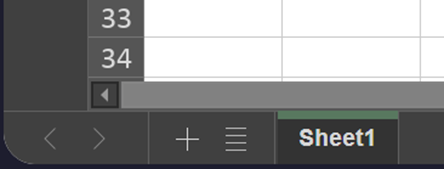
\includegraphics[width=\textwidth]{_Aufgaben/img/A02_newSheet.png}
    }
}
